\newpage

\section{Region-Based Analysis}

The iterative data-flow analysis algorithm we have discussed so far is just one approach to solving data-flow problems.
Here we discuss another approach called region-based analysis\cite{Microsof22:online}. Recall that in the iterative-analysis approach,
we create transfer functions for basic blocks, then find the fixedpoint solution by repeated passes over the blocks.
Instead of creating transfer functions just for individual blocks, a region-based analysis finds transfer functions that
summarize the execution of progressively larger regions of the program. Ultimately, transfer functions for entire procedures are constructed
and then applied, to get the desired data-flow values directly.



While a data-flow framework using an iterative algorithm is specified by a semilattice of data-flow values and a family of transfer
functions closed un-der composition, region-based analysis requires more elements. A region-based framework includes both a semilattice
of data-flow values and a semilattice of transfer functions that must possess a meet operator, a composition operator,
and a closure operator.

A region-based analysis is particularly useful for data-flow problems where paths that have cycles may change the data-flow values.
The closure operator allows the effect of a loop to be summarized more effectively than does iterative analysis.
The technique is also useful for interprocedural analysis, where transfer functions associated with a procedure call may be treated like
the transfer functions associated with basic blocks.

\subsection{Motivating Example}

Consider the example in \ref{fig:p115}, we want to know how many bits needed to store the return value for a fpga device. We can pessimistically solve for the worst case.
But we can also try to be more precise to calculate for each call site. It would be nice if instead of having to go back and iteratively solve a problem, for each different value of x.


\begin{figure}[H]
	\centering
	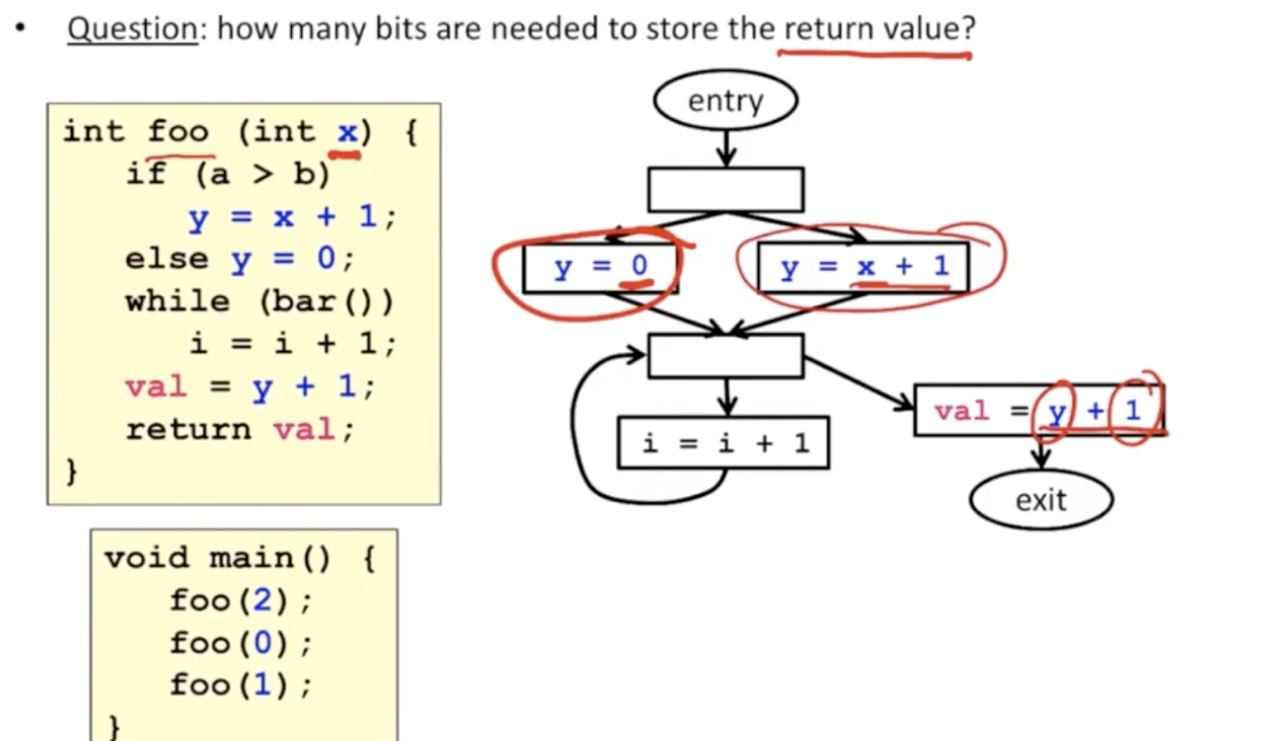
\includegraphics[width=0.5\textwidth]{p115.jpg}
	\caption{Motivating Example for region-based analysis}
	\label{fig:p115}
\end{figure}

The idea behind region-based analysis is that we want to create a transfer function for the entire procedure.



\subsection{Algorithm}


\begin{definition}{Region}
	A region in a flow graph is
	a set of nodes with a
	header that dominates all
	other nodes in a region.
\end{definition}

In Iterative Analysis, {\color{blue}Transfer function}
	{\color{red}\(F_B\)}
summarize effect from {\color{blue}beginning to end of basic block B}.

In Region-Based Analysis, {\color{blue}Transfer function}
	{\color{red}\(F_{R,B}\)}
summarize effect from {\color{blue}beginning of region
			{\color{red}R} to end of basic block B}. Recursively
construct a larger region  {\color{red}R} from smaller regions
construct {\color{red}\(F_{R,B}\)} from transfer functions for smaller
regions
until the program is one region.
Let P be the region for the entire program,
and v be initial value at entry node, {\color{blue}out[B] = {\color{red}\(F_{R,B}\)} (v)},
{\color{blue}in[B] = {\color{red}\( \cap_{B^\prime}out[B^\prime] \)}} where B’ is a predecessor of B


We will use Reaching definitions as our transfer function to illustrate Region-Based Analysis.


\subsubsection{Operations on Transfer Functions}

\begin{figure}[H]
	\centering
	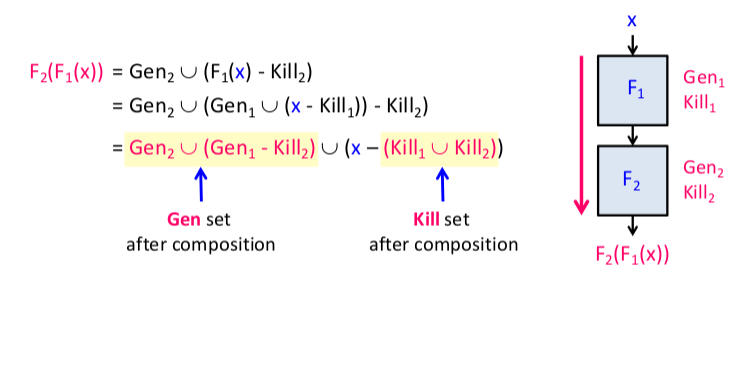
\includegraphics[width=0.7\textwidth]{p116.png}
	\caption{Operations on Transfer Functions: Composition}
	\label{fig:p116}
\end{figure}

\begin{figure}[H]
	\centering
	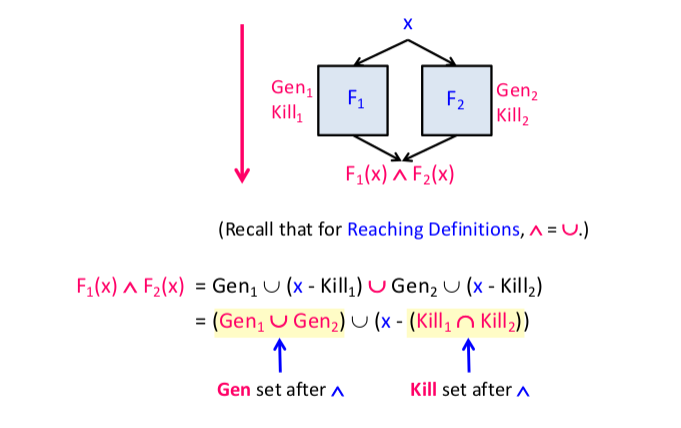
\includegraphics[width=0.7\textwidth]{p117.png}
	\caption{Operations on Transfer Functions: Meet}
	\label{fig:p117}
\end{figure}

\begin{figure}[H]
	\centering
	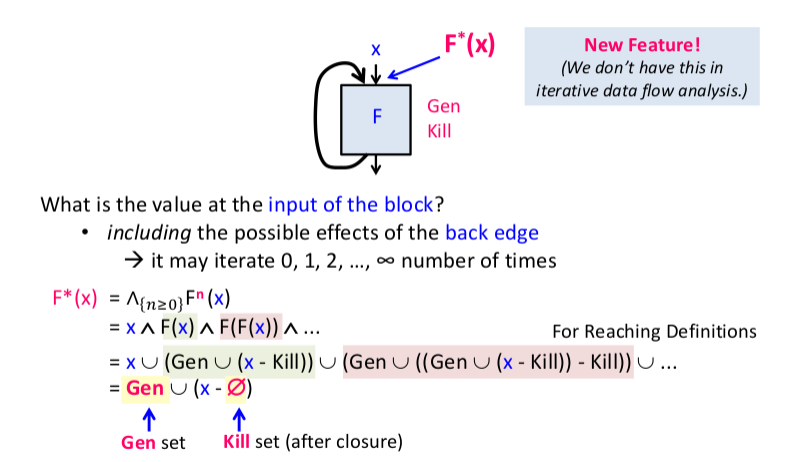
\includegraphics[width=0.7\textwidth]{p118.png}
	\caption{Operations on Transfer Functions: Closure}
	\label{fig:p118}
\end{figure}



\subsubsection{Structure of Nested Regions (An Example)}

\begin{figure}[H]
	\centering
	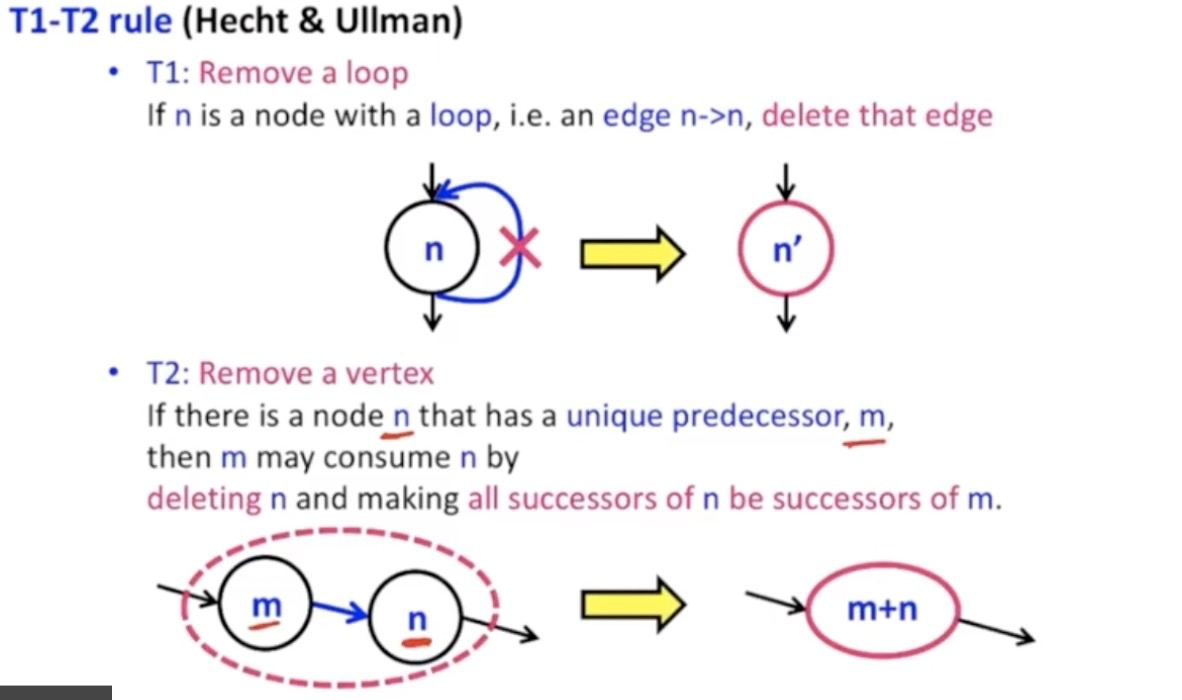
\includegraphics[width=0.7\textwidth]{p119.jpg}
	\caption{}
	\label{fig:p119}
\end{figure}


\subsubsection{Transfer Functions for T2 Rule}

\begin{figure}[H]
	\centering
	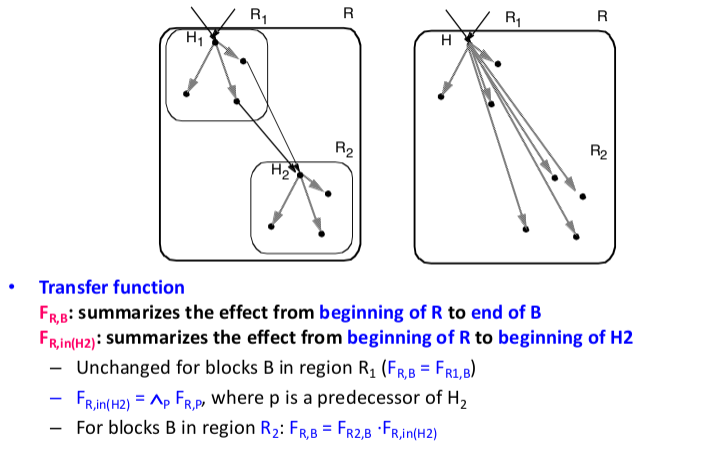
\includegraphics[width=0.7\textwidth]{p121.png}
	\caption{}
	\label{fig:p121}
\end{figure}



\subsubsection{Transfer Functions for T1 Rule}


\begin{figure}[H]
	\centering
	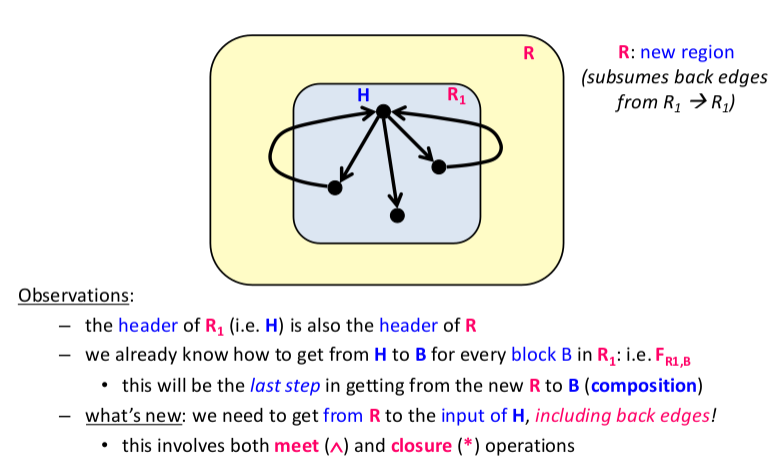
\includegraphics[width=0.7\textwidth]{p120.png}
	\caption{}
	\label{fig:p120}
\end{figure}


\subsubsection{Example: Reaching Definitions}

\begin{figure}[H]
	\centering
	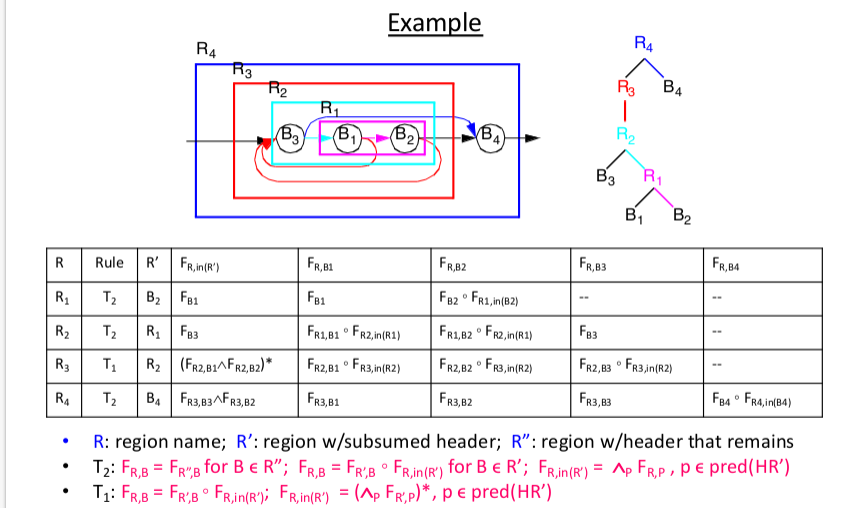
\includegraphics[width=0.7\textwidth]{p126.png}
	\caption{}
	\label{fig:p126}
\end{figure}



\begin{figure}[H]
	\centering
	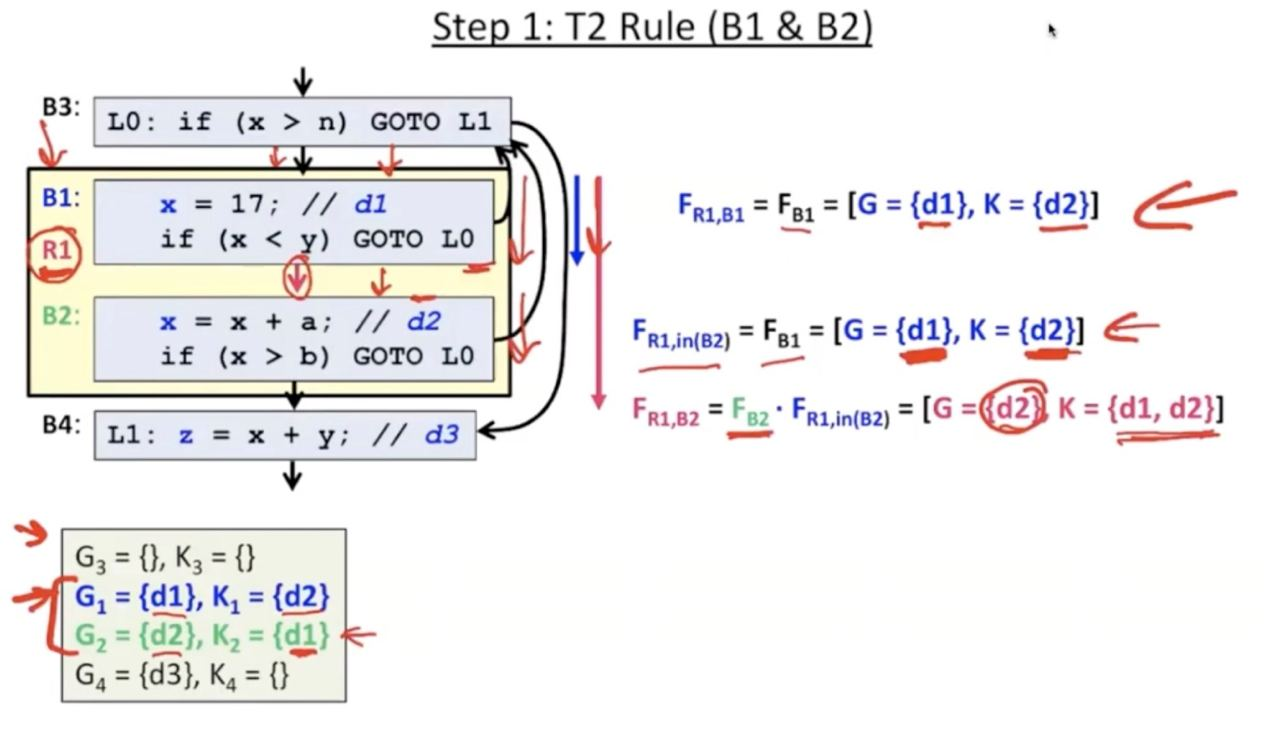
\includegraphics[width=0.7\textwidth]{p122.jpg}
	\caption{}
	\label{fig:p122}
\end{figure}

\begin{figure}[H]
	\centering
	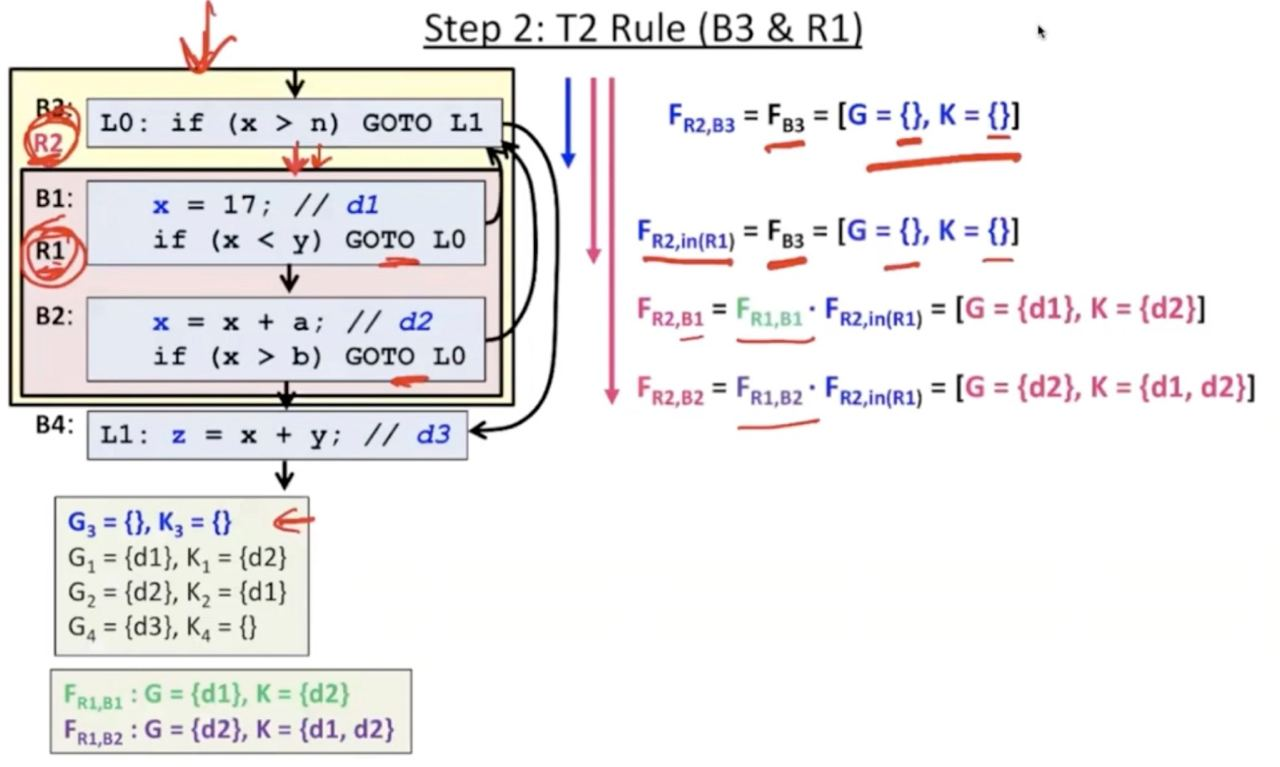
\includegraphics[width=0.7\textwidth]{p123.jpg}
	\caption{}
	\label{fig:p123}
\end{figure}
\begin{figure}[H]
	\centering
	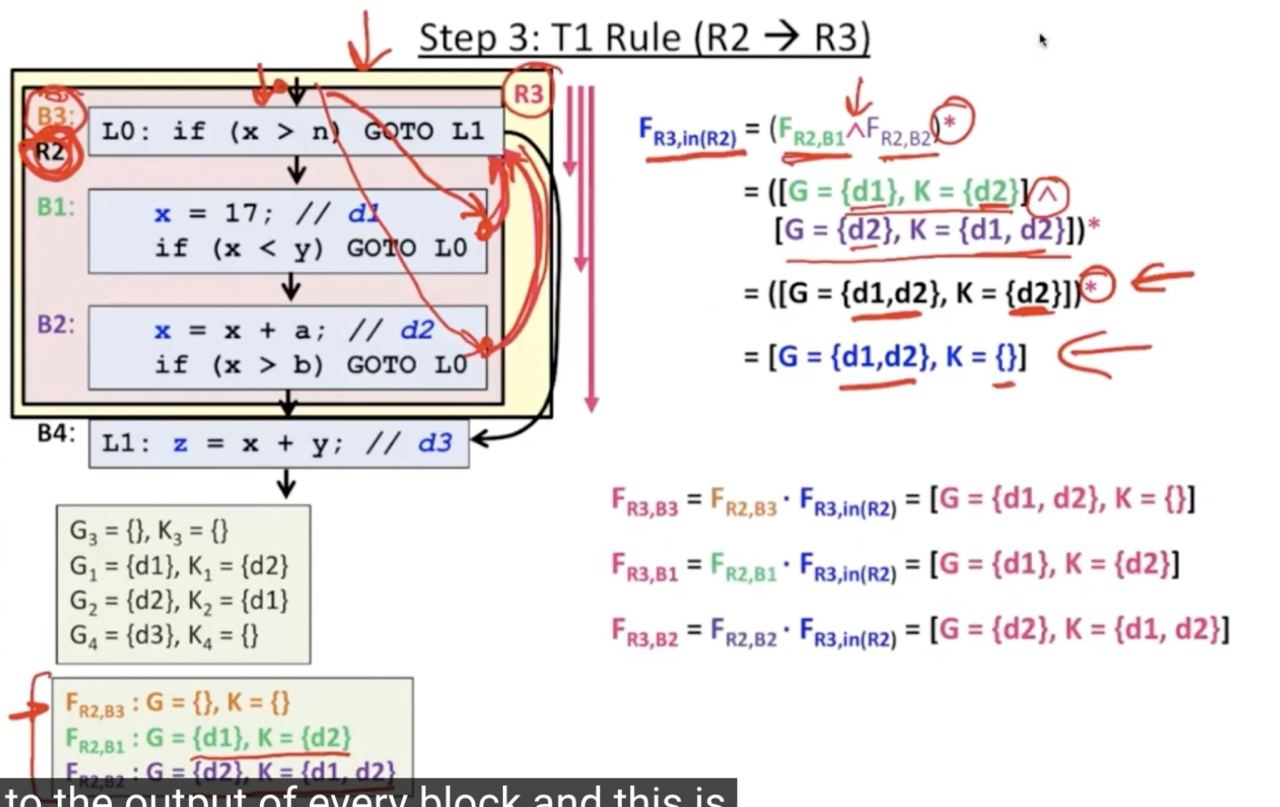
\includegraphics[width=0.7\textwidth]{p124.jpg}
	\caption{}
	\label{fig:p124}
\end{figure}
\begin{figure}[H]
	\centering
	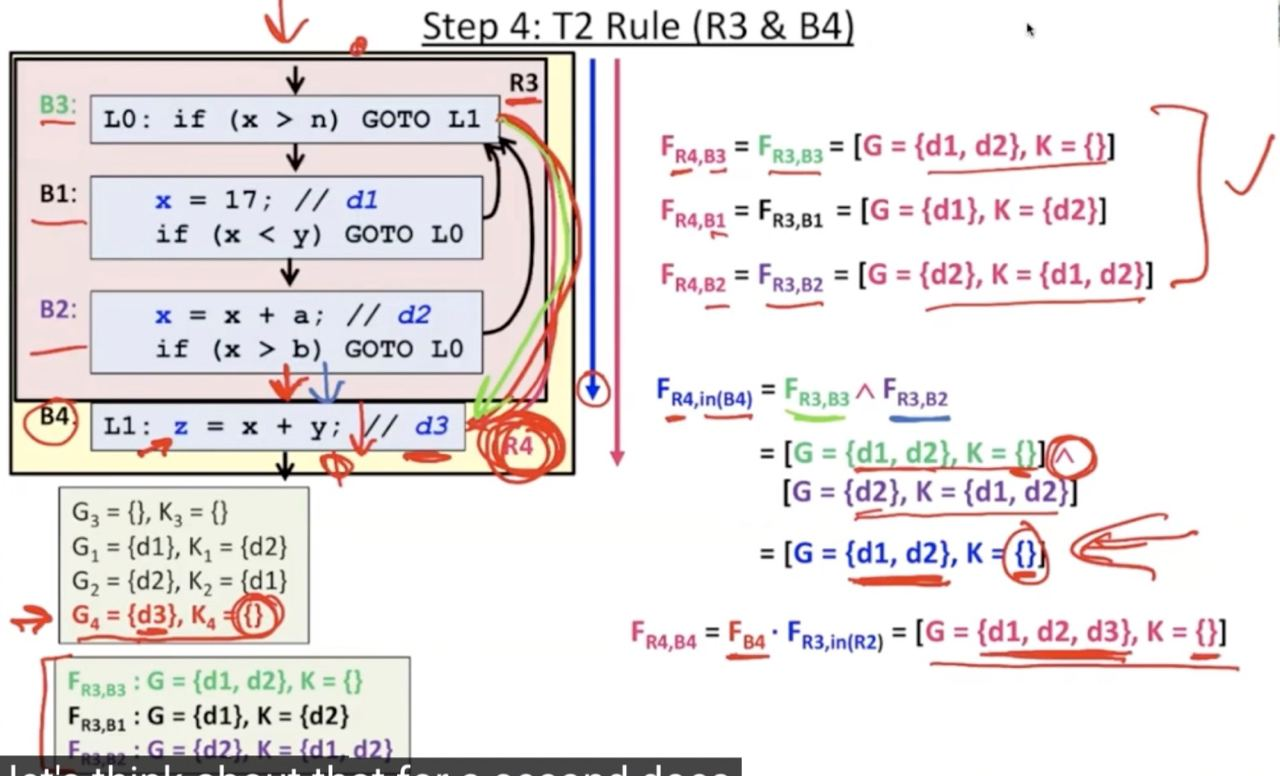
\includegraphics[width=0.7\textwidth]{p125.jpg}
	\caption{}
	\label{fig:p125}
\end{figure}
